\documentclass[a4paper]{report}
\usepackage[utf8]{inputenc}
\usepackage[spanish]{babel}
\usepackage[dvipsnames]{xcolor}
\usepackage{parskip}
\usepackage[colorlinks=true,urlcolor=blue,linkcolor=black]{hyperref}
\usepackage{url}
\usepackage{booktabs}
\usepackage{float}
\usepackage{adjustbox}
\usepackage{amsmath,amssymb}
\usepackage{graphicx}
\usepackage{geometry}
\usepackage{subfig}
\usepackage{caption}
\usepackage{wrapfig}
\usepackage{float}
\usepackage{multicol}
\usepackage{tcolorbox}
\usepackage{fancyvrb}
\usepackage{booktabs}
\usepackage{multirow}
\usepackage{lmodern}
\usepackage{color,array}
\usepackage{etoolbox}
\usepackage{minted}

\makeatletter
\patchcmd{\@makechapterhead}{\vspace*{50\p@}}{}{}{}% Removes space above \chapter head
\patchcmd{\@makeschapterhead}{\vspace*{50\p@}}{}{}{}% Removes space above \chapter* head
\makeatother

\unaccentedoperators

\setlength{\textfloatsep}{0pt}
\counterwithout{section}{chapter}
\usemintedstyle{murphy}

\title{\Huge{}\texttt{MIPS R2000}\\\vspace{8pt}\Large{}\textbf{\scalebox{.85}[1.0]{Práctica 1}}}
\author{Ariel Leonardo Fideleff}

\begin{document}

\pagenumbering{gobble}
\maketitle

\chapter{Cuestiones}

\section{Apartado 1}

\begin{center}
\large\textbf{-- \textsl{Declaración de palabras en memoria} --}
\end{center}

\subsection*{1.1 y 1.2}

Como podemos ver en la Figura \ref{fig:c1-1}, los dos números enteros reservados en el programa se ubicaron en las posiciones \texttt{0x10010000} y \texttt{0x10010004}, distanciados justamente por 4 bytes ya que se corresponde con el tamaño de palabra. Es decir, si cada entero fue reservado como un \mintinline{gas}{.word}, cada uno ocupa 4 bytes. Con esto, sumado a que el ensamblador los coloca uno seguido del otro en la memoria, dado que el primer valor por defecto comienza en la posición \texttt{0x10010000}, el segundo necesariamente deberá ubicarse 4 posiciones de memoria después (cada posición se corresponde con un byte).

En cuanto a los valores como tal, podemos ver la diferencia en que hayamos indicado uno en decimal, mientras el otro en hexadecimal. De esta forma, el número 15 en decimal es representado como \texttt{0x0000000f} en hexa, forma con la cual se presenta en el panel de datos. Mientras, el segundo valor, al haber sido especificado en el programa en base 16, lo reconocemos fácilmente como \texttt{0x00000015} en el panel en cuestión.

\begin{figure}[h]
    \centering
    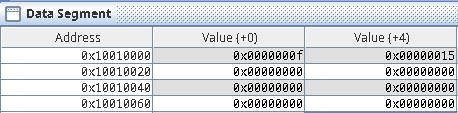
\includegraphics[width=.7\linewidth]{img/c1-1}
    \caption{Datos del programa según se indican en el panel de datos}
    \label{fig:c1-1}
\end{figure}

\subsection*{1.3}

De acuerdo a lo dicho en la teoría, las etiquetas \texttt{palabra1} y \texttt{palabra2} deberían tomar el valor de las posiciones de memoria a las que hacen referencia. En este caso, las ya mencionadas \texttt{0x10010000} y \texttt{0x10010004}, respectivamente.

De hecho, como se muestra en la Fig. \ref{fig:labels-fst}, esto lo podemos comprobar en la ventana \textit{Labels}, que se puede activar desde la configuración del simulador.

\begin{figure}[h]
    \centering
    \captionsetup{justification = centering}
    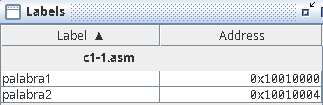
\includegraphics[width=.5\linewidth]{img/c1-3}
    \caption{Valores de las etiquetas \texttt{palabra1} y \texttt{palabra2} en la ventana \textit{Labels}}
    \label{fig:labels-fst}
\end{figure}

\subsection*{1.4}

Al ensamblar el programa dado, no parece presentar ninguna diferencia con respecto al primer programa visto, ya sea tanto en la memoria, como también en otras variables visibles en el simulador (por ejemplo, los registros).

\subsection*{1.5}

El siguiente código cumple con la consigna planteada:

\vspace{7pt}
\inputminted[linenos]{gas}{src/cuestiones/c1-5.asm}
\vspace{7pt}

Y en la Figura \ref{fig:arr5-mem} podemos comprobar que los valores fueron almacenados de forma correcta, considerando que los números 30 y 60 en decimal se corresponden con \texttt{0x0000001e} y \texttt{0x0000003c} en hexadecimal, respectivamente.

\begin{figure}[h]
    \centering
    \captionsetup{justification = centering}
    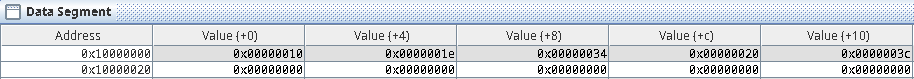
\includegraphics[width=.95\linewidth]{img/c1-5a}
    \caption{Valores del vector de números declarado en el programa propuesto, según se indican en el panel de datos}
    \label{fig:arr5-mem}
\end{figure}

Notar que al haber cambiado la dirección de memoria inicial donde se quiere que se almacenen los datos (respecto a la utilizada por defecto), debimos de expandir el panel de datos del simulador para poder visualizar el segmento de la memoria donde se ubicaban los valores reservados de nuestro vector, seleccionando la opción correspondiente desde un menú desplegable, tal como se lo muestra en la Figura \ref{fig:dropdown-data}.


\begin{figure}[h]
    \centering
    \captionsetup{justification = centering}
    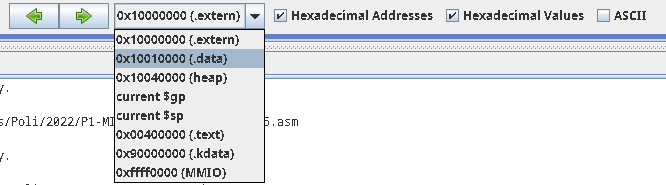
\includegraphics[width=.7\linewidth]{img/c1-5b}
    \caption{Menú desplegable para seleccionar la visualización del segmento de memoria correspondiente al utilizado por el programa planteado}
    \label{fig:dropdown-data}
\end{figure}

\subsection*{1.6}

Podemos probar cambiar el argumento de la directiva \mintinline{gas}{.data} para intentar almacenar los datos partiendo desde la dirección \texttt{0x10000002}:

\vspace{7pt}
\inputminted[linenos]{gas}{src/cuestiones/c1-6.asm}
\vspace{7pt}

Hecho este cambio, el panel de datos nos muestra que los valores ahora son almacenados partiendo desde la dirección de memoria \texttt{0x10000004}, saltando de 4 en 4 (por el tamaño de palabra, Fig. \ref{fig:not-multiple}).

\begin{figure}[h]
    \centering
    \captionsetup{justification = centering}
    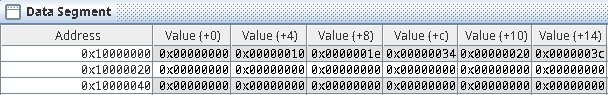
\includegraphics[width=.8\linewidth]{img/c1-6}
    \caption{Valores y respectivas posiciones de memoria del programa con argumento de \mintinline{gas}{.data} modificado}
    \label{fig:not-multiple}
\end{figure}

Esto difiere en principio de lo que uno podría esperar, ya que se le está indicando al ensamblador que ubique la información partiendo desde la dirección de memoria \texttt{0x10000002}. El motivo por el cual ejecuta el cambio descripto, es porque se requiere que la ubicación de todos los valores se encuentren en posiciones múltiplos de 4, de forma que la memoria ``esté alineada''. Éste es un requisito de la arquitectura MIPS, o bueno, al menos estamos seguros basándonos en lo visto en la teoría, que lo es para el lenguaje de máquina de los microprocesadores MIPS R2000.

Con esto en cuenta, el ensamblador, sabiendo que indicamos el espacio para datos partiendo desde la posición de memoria \texttt{0x10000002}, buscó por la posición de memoria (mayor o igual) múltiplo de 4 más cercana, y a partir de allí ubicó los valores del vector de números reservado en el programa.

\begin{center}
\large\textbf{-- \textsl{Declaración de bytes en memoria} --}
\end{center}

\subsection*{1.7 y 1.8}

\begin{wrapfigure}[11]{r}{.25\linewidth}
    \centering
    \captionsetup{justification = centering}
    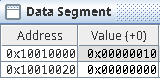
\includegraphics[width=\linewidth]{img/c1-7}
    \caption{Representación del contenido especificado en la memoria, visto desde el panel de datos}
    \label{fig:c1-7}
\end{wrapfigure}

Como ya sabemos, al no especificar ningún argumento para la directiva \mintinline{gas}{.data}, los datos se ubicarán partiendo desde la dirección de memoria \texttt{0x10010000} por defecto.

Además, al tratarse de un único byte, y considerando que el valor indicado \texttt{0x10} no supera el tamaño permitido por la directiva (el máximo valor posible sería \texttt{0xFF}), éste se almacenaría ``al comienzo de la palabra'', efectivamente implicando que el valor de la palabra que contiene el byte sea el mismo al especificado. Al fin y al cabo, el tamaño de una palabra es mayor al de un byte (justamente, 4 bytes), por lo que resulta en que el valor de la palabra sea el mismo al valor del tamaño de un byte, antecedido por 0s que no cambian el entero final almacenado.

\subsection*{1.9 y 1.10}

En este caso, se almacenan los valores \textbf{\texttt{0x40302010}} y \textbf{\texttt{0x10203040}} en las posiciones de memoria \textbf{\texttt{0x10010000}} y \textbf{\texttt{0x10010004}} respectivamente.

Si bien el segundo valor es indicado como tal de forma explícita en el código presentado, el primer valor, en cambio, es el resultado de almacenar un vector de 4 valores especificados del tamaño de 1 byte. Esto nos muestra que el simulador, por un lado, almacena los valores indicados con la directiva \mintinline{gas}{.byte} de forma contigua, independientemente de que los valores sean accedidos de a una palabra a la vez. Por otro lado, nos indica también el orden que utiliza para guardar los datos dentro de una palabra, el cual puede ser identificado afín con el concepto de \textit{Little-Endian}, el cual consiste en la organización y alineamiento de los datos de forma que, aplicado a este caso, ``lo que va primero'' se almacene en las direcciones de memoria más bajas, y así en adelante.\footnote{Más formalmente, el concepto de \textit{Little Endian} hace referencia a que los bytes menos significativos dentro de una palabra sean almacenados en posiciones de memoria más chicas, relacionándose principalmente con la forma en la que se \textit{internamente} se manejan y ordenan los bytes de una palabra.}

Esta conclusión la podemos obtener partiendo, primero, en que sabemos que el valor presentado en el panel de datos de una palabra \texttt{0xXXXXXXXX}, se corresponde con la representación en hexadecimal de los bytes en posiciones de memoria menores a mayores, interpretadas de derecha a izquierda. Para probar esto, podemos modificar el programa descripto para la consigna, y especificar que los datos se ubiquen partiendo desde la dirección de memoria \texttt{0x10010002}:

\vspace{7pt}
\inputminted[linenos]{gas}{src/cuestiones/c1-10.asm}
\vspace{7pt}

Con este cambio, la palabra en la dirección \texttt{0x10010000} almacena ahora el valor \texttt{0x20100000}, a la vez que la palabra en la dirección \texttt{0x10010004} almacena los dos valores restantes del vector de \mintinline{gas}{.byte} (valor \texttt{0x00004030}, ver Fig. \ref{fig:bytes-shift-endian}), demostrando cómo los bytes se corrieron dos posiciones desde la derecha (posiciones como bytes, que en hexadecimal se corresponde con dos dígitos, así representando un espacio de 4 dígitos para haber cambiado la dirección de memoria de \mintinline{gas}{.data} dos posiciones adelante de la usada por defecto).

\begin{figure}[h]
    \centering
    \captionsetup{justification = centering}
    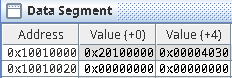
\includegraphics[width=.4\linewidth]{img/c1-10}
    \caption{Valores de las palabras en memoria correspondientes al vector de \mintinline{gas}{.byte}, tras indicar que los datos se almacenen desde la posición \texttt{0x10010002}}
    \label{fig:bytes-shift-endian}
\end{figure}

Teniendo esto en cuenta, vemos que los valores del vector de \mintinline{gas}{.byte} fueron almacenados en orden creciente respecto a posiciones de memoria que también crecen. Así, como en el programa indicamos los números \texttt{0x10}, \texttt{0x20}, \texttt{0x30} y \texttt{0x40} (en este orden), el primero de todos, el \texttt{0x10}, se encuentra en la posición de memoria \texttt{0x10010000}, luego el \texttt{0x20} en la posición \texttt{0x10010001}, y así sucesivamente.

Por ende, leemos el vector completo como el valor de una palabra \texttt{0x40302010} (siendo 4 elementos, exactamente la misma cantidad como hay de bytes en una palabra, siendo una sola suficiente para representar la totalidad de dicho vector). Mientras, guardar el valor \texttt{0x10203040} nos da una la pauta de cómo se hubieran almacenado los valores del vector en cuestión si el ensamblador hubiera tenido un comportamiento que se acercara a \textit{Big-Endian} (en el cual los ``últimos números'' se guardarían en las posiciones de memoria más pequeñas/bajas).

\subsection*{1.11}

A pesar del comportamiento de juntar los valores del tamaño de 1 byte en palabras, esto no afecta sobre los valores de las etiquetas \texttt{palabra1} y \texttt{palabra2}, que indican la primera posición de memoria desde la cual parte cada valor (en este caso, digamos, el vector y el segundo valor). Además, ayuda que puntualmente el vector definido en la consigna pueda estar contenido en una sola palabra, como ya mencionamos.

Por lo tanto, las etiquetas \texttt{palabra1} y \texttt{palabra2} toman los valores \texttt{0x10010000} y \texttt{0x10010004} respectivamente.

\begin{center}
\large\textbf{-- \textsl{Declaración de cadenas de caracteres} --}
\end{center}

\end{document}
